\documentclass[11pt,a4paper]{report}      %% LaTeX2e document.
\usepackage{graphicx, tabularx}
\usepackage{rotating}
\usepackage[round]{natbib}  
\begin{document}
\section{Abstract}
CSS081231:071126+440405 is an eclipsing polar with a period of 117 minutes. Small and medium sized telescopes have photometry of the system dating back to late 2008. The ephemeris was computed shortly after discovery and then revised recently following five years of subsequent observations. Newer photometric observations have allowed us to place tighter contraints on the orbital parameters. We have obtained six optical spectra of the system covering phases 0.24 to 0.90. The spectra show clear cyclotron humps, revealing magnetic field strength of $B  \sim 35 MG$.

\section{Schwope paper}

\section{Introduction}


\section{Data}
6 nights of photometry were obtained using ULTRASPEC \citep{ULTRASPEC}, mounted on the 2.5m Thai National Telescope during 2014 and 2015. The details for these nights is shown in table \ref{tab:photometry}. The data has been phase folded using the ephemeris given by \citet{Schwope2015} which is 
\begin{equation}BJD(TDB) = 2454833.207868(14) + E\times0.0813768094(6)\end{equation}

\begin{table}
  \caption{Photometry used in this study. The instrument used was ULTRASPEC, mounted on the Thai National Telescope at the Thai National Observatory.}
  \begin{tabularx}{\textwidth}{ l  l  l  l  l  }
  \hline
  Instrument & Date & Filter & $T_{exp}$& Total time \\
  \hline
    TNT - ULTRASPEC & 2014/02/06 & KG5 & 1.5s & 147.8m \\
    TNT - ULTRASPEC & 2014/02/07 & KG5 & 1.7s & 166.2m \\
    TNT - ULTRASPEC & 2014/02/08 & KG5 & 2.8s & 73.6m \\
    TNT - ULTRASPEC & 2014/12/12 & KG5 & 3.0s? & 95.1m \\
    TNT - ULTRASPEC & 2015/01/01 & KG5 & 2.0s & 118.2m \\
    TNT - ULTRASPEC & 2015/01/03 & KG5 & 2.0s & 131.1m \\
    
  \hline
  \end{tabularx}
  \label{tab:photometry}
\end{table}

\begin{sidewaysfigure}[ht]
\centering
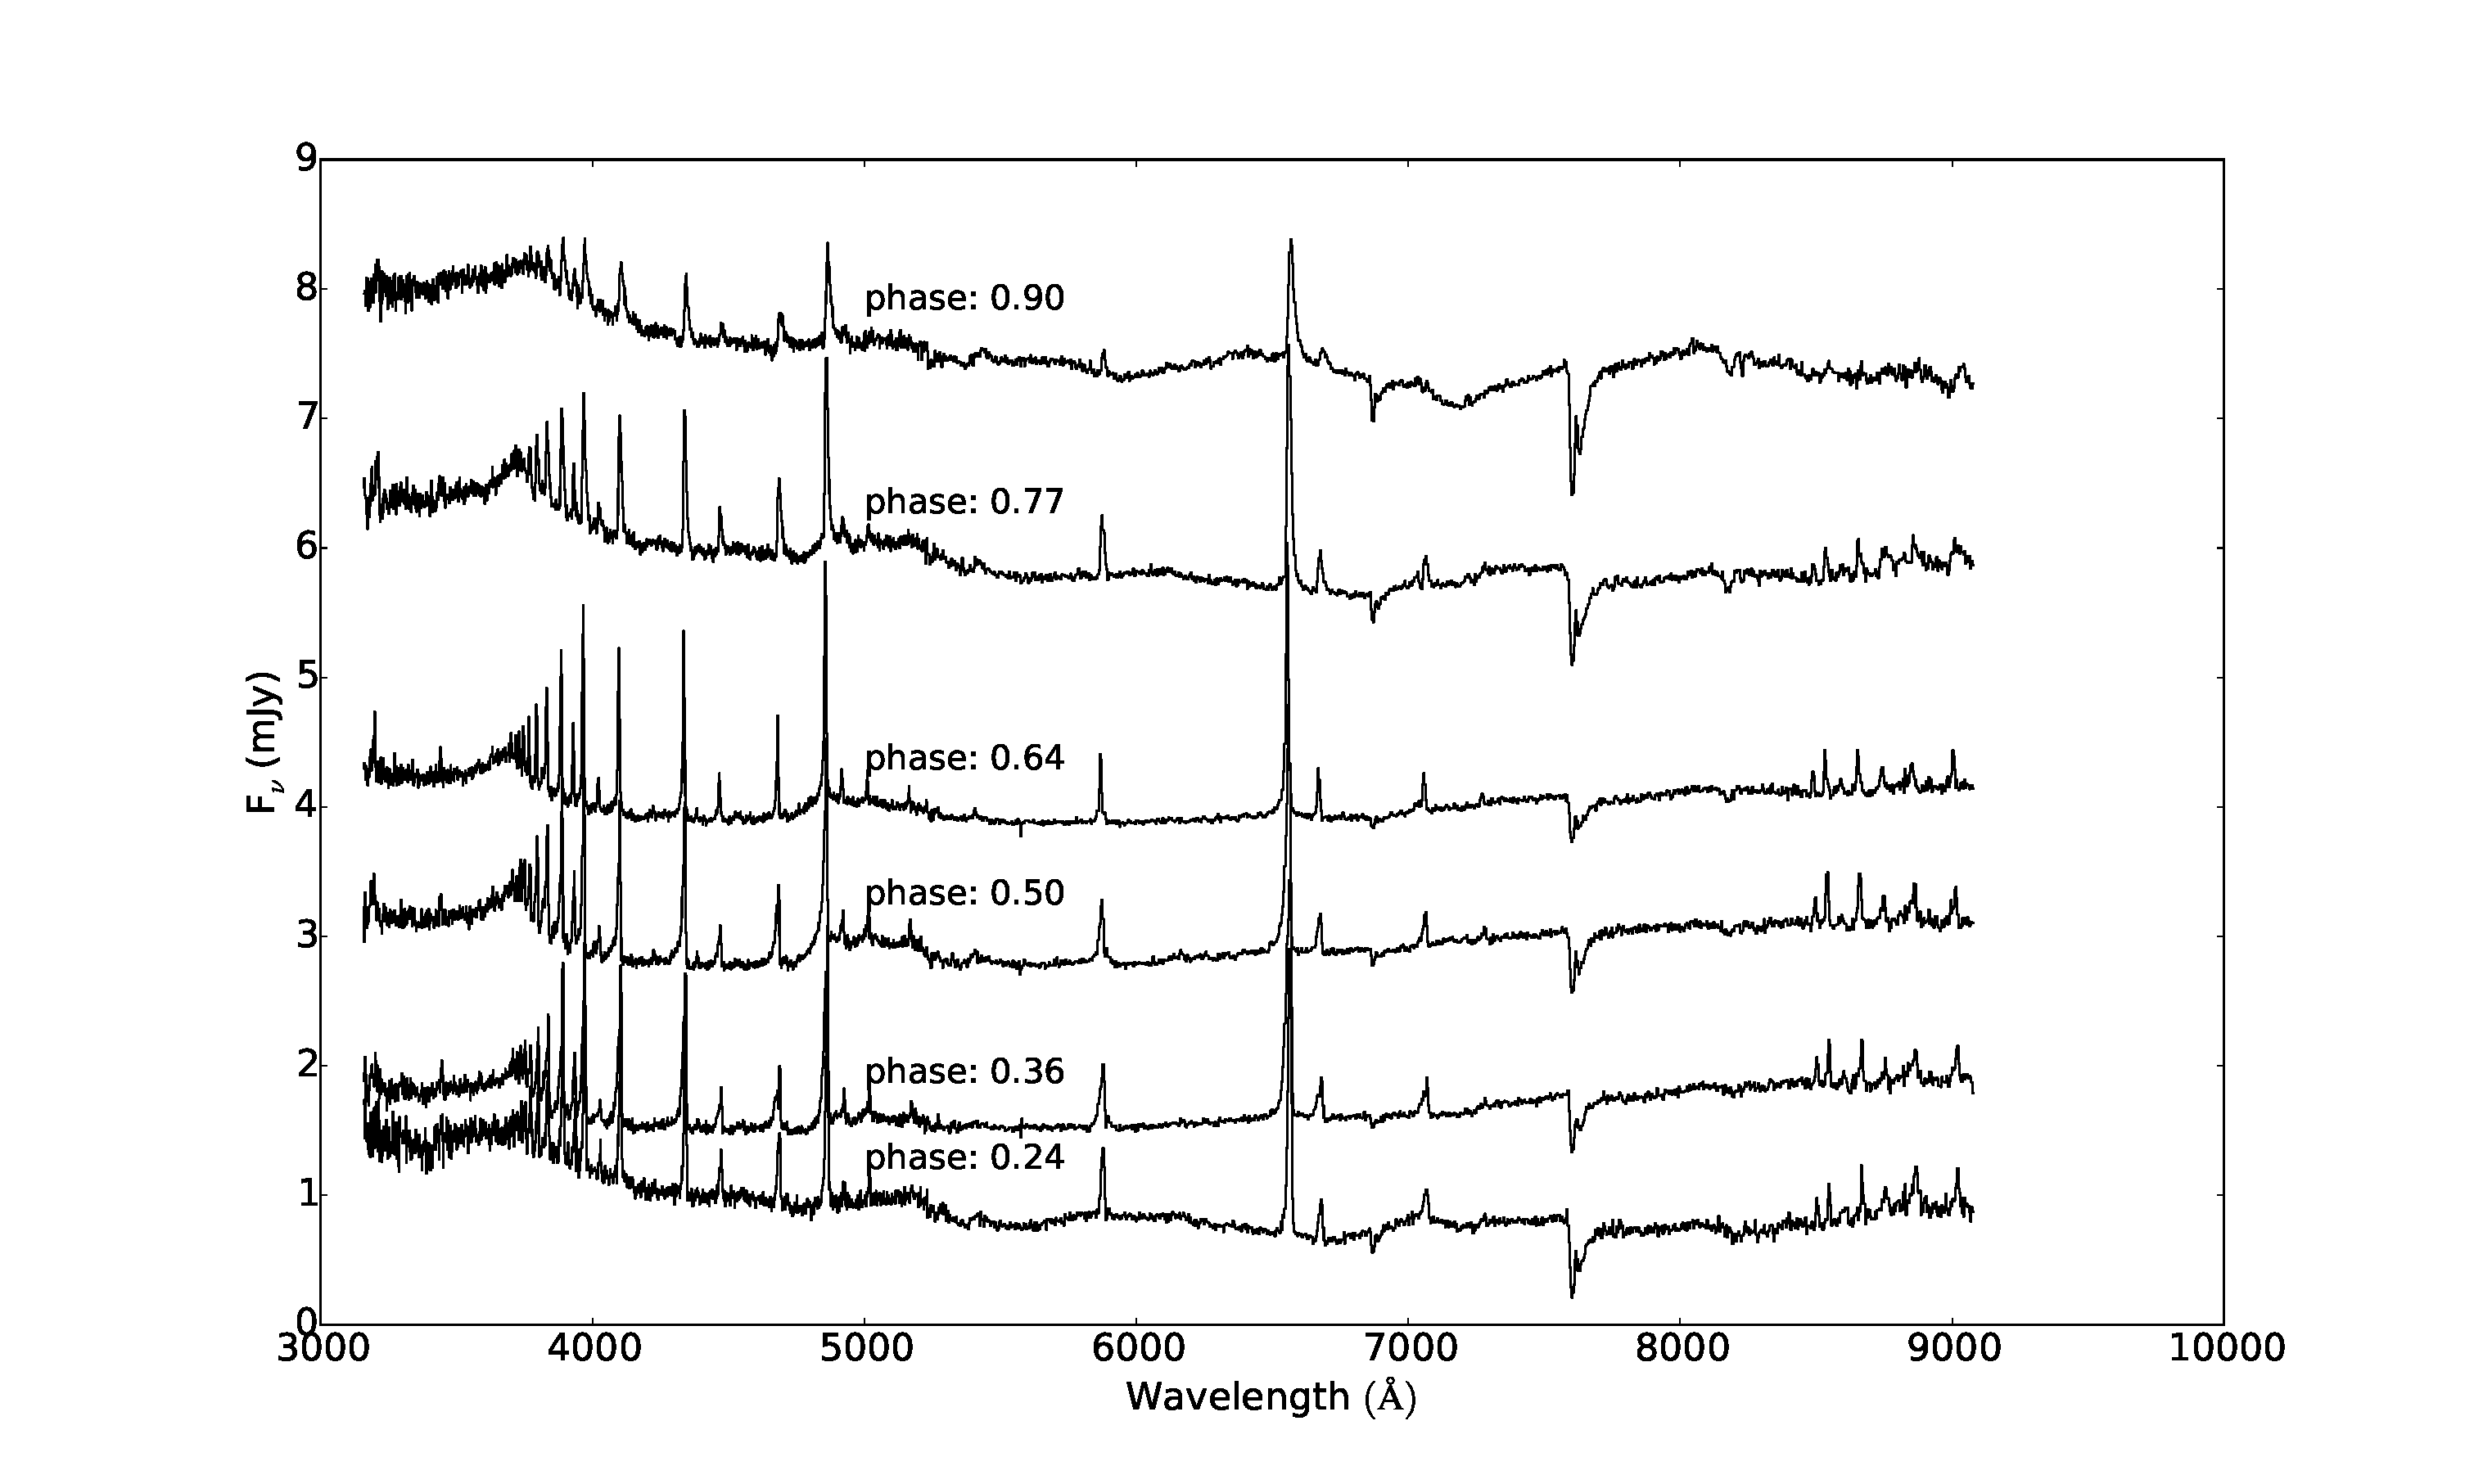
\includegraphics[width=\textwidth]{images/CSS081231_spectra.eps}
\caption[Caption for spectra]{The optical spectra of CSS081231 taken at 6 stages of the orbital cycle. Cyclotron humps are seen in the early and late stages of the orbit when the accretion stream is in view. During the mid-phases of the orbit the accretion stream is eclipsed by the white dwarf. }
\label{fig:spectra}
\end{sidewaysfigure}

\section{Discussion}

\section{Conclusion}


\bibliographystyle{plainnat}

\bibliography{rashley}            %% Start your bibliography here;
                                 %! with sample.bib as your bibliography file. You can
                               %% also use:
                %! \begin{thebibliography}

\end{document}